%%%%%%%%%%%%%%%%%%%%%%%%%%%%%%%%%%%%%%%%%
% Simple Sectioned Essay Template
% LaTeX Template
% i
% This template has been downloaded from:
% http://www.latextemplates.com
%
% Note:
% The \lipsum[#] commands throughout this template generate dummy text
% to fill the template out. These commands should all be removed when 
% writing essay content.
%
%%%%%%%%%%%%%%%%%%%%%%%%%%%%%%%%%%%%%%%%%

%----------------------------------------------------------------------------------------
%	PACKAGES AND OTHER DOCUMENT CONFIGURATIONS
%----------------------------------------------------------------------------------------

\documentclass[12pt]{article} % Default font size is 12pt, it can be changed here
\usepackage[english]{babel}
\usepackage[square,sort,comma,numbers]{natbib}
\usepackage[utf8]{inputenc}
\usepackage{listings}
\usepackage{color}
\usepackage{caption}
\usepackage[dvips]{graphicx}
\usepackage{geometry} % Required to change the page size to A4
%\geometry{a4paper} % Set the page size to be A4 as opposed to the default US Letter
\usepackage{framed}
\usepackage{graphicx} % Required for including pictures
\usepackage{amssymb}
\usepackage{url}

\usepackage{float} % Allows putting an [H] in \begin{figure} to specify the exact location of the figure
\usepackage{wrapfig} % Allows in-line images such as the example fish picture

\usepackage{fancyhdr}
\pagestyle{fancy}
\fancyhf{}
\fancyhead[RO]{{Assignment - 3}} 
\fancyhead[LO]{Biomedical Image Processing}
%\fancyhead[RO]{{\leftmark}} 
\fancyfoot[LE,RO]{{ \thepage }}

%\usepackage{lipsum} % Used for inserting dummy 'Lorem ipsum' text into the template
\definecolor{grey}{rgb}{0.9,0.9,0.9}

\linespread{1.2} % Line spacing

%\setlength\parindent{0pt} % Uncomment to remove all indentation from paragraphs

\graphicspath{{./Pictures/}} % Specifies the directory where pictures are stored
\newcounter{ejercicioNo}
\begin{document}

%----------------------------------------------------------------------------------------
%	TITLE PAGE
%----------------------------------------------------------------------------------------

\begin{titlepage}

\newcommand{\HRule}{\rule{\linewidth}{0.5mm}} % Defines a new command for the horizontal lines, change thickness here

\center % Center everything on the page

\textsc{\LARGE Universidad Aut\'{o}noma de Madrid}\\[1.5cm] % Name of your university/college
%\textsc{\Large Proyecto de Sistemas Informaticos}\\[0.5cm] % Major heading such as course name
%\textsc{\large Departamento de Informatica}\\[0.5cm] % Minor heading such as course title
\textsc{\Large Computer Science Department}\\[0.5cm] % Minor heading such as course title

\HRule \\[0.4cm]
{ \huge \bfseries Biomedical Image Processing\\[0.5cm] Assignment - 3}\\[0.4cm] % Title of your document
\HRule \\[1.5cm]

%\begin{minipage}{0.4\textwidth}
%\begin{flushleft}
% \large
%\emph{Author:}\\
%Roberto  \textsc{Marabini Ruiz} % Your name
%\end{flushleft}
%\end{minipage}

%\begin{minipage}{0.4\textwidth}
%\begin{flushright} \large
%\emph{Supervisor:} \\
%Dr. James \textsc{Smith} % Supervisor's Name
%\end{flushright}
%\end{minipage}\\[4cm]

%{\large \today}\\[3cm] % Date, change the \today to a set date if you want to be precise

%\includegraphics{Logo}\\[1cm] % Include a department/university logo - this will require the graphicx package

\vfill % Fill the rest of the page with whitespace
%\begin{minipage}{0.4\textwidth}
\begin{flushright}
 \large
%\emph{Author:}\\
Roberto  \textsc{Marabini Ruiz} % Your name
\end{flushright}
%\end{minipage}

\end{titlepage}

%----------------------------------------------------------------------------------------
%	TABLE OF CONTENTS
%----------------------------------------------------------------------------------------

\tableofcontents % Include a table of contents

\newpage % Begins the essay on a new page instead of on the same page as the table of contents 

%----------------------------------------------------------------------------------------
%	OBJETIVOS
%----------------------------------------------------------------------------------------

\section {Goal}

In this assignment we will explore a 3D reconstruction algorithm based on expectation maximization and maximum likelihood (EM-ML) for three dimensional reconstruction of PET data. This is a crucial equation for PET tomography and over the past 30 years, much of the work in statistically based algorithms has been concentrated on finding alternative implementations of this EM-ML algorithm that converge faster or offer improved resolution, contrast and/or signal-to-noise ratio. 

%------------------------------------------------
\section{Introduction} % Sub-section

In a PET study, a biochemical metabolite labeled with a positron emitting radioactive material is introduced into the body under study and the radioactive emissions are then counted using a PET scanner. The physics behind this phenomenon is as follows: when a positron is emitted, it “finds” a nearby electron and annihilates with it. The annihilation creates two gamma photons that fly off the point of annihilation, in (nearly) opposite directions along a line with completely random (i.e uniformly distributed in space) orientation. The line defined by the two opposite photons is usually referred to as line of response (LOR). A PET machine consists of an array of detector elements surrounding the body, and the two photons are detected in coincidence by a pair of these detector elements.

Vardi et al. \cite{Vardi1985} developed an algorithm to estimate the spatial distribution of the 
radioactive material from a set of measurements acquired by discrete bin detectors. Their mathematical 
development starts by assuming that positron emissions occur according to a spatial Poisson point 
process in a certain region $\mathbb{R}^{3}$ 
with an unknown intensity function  $\lambda(\mathbf{r})$. 
The measured data set is the total number of coincidences along each LOR. In its list-mode version 
\cite{Reader1998} the 3D reconstruction iterative method has the form.

\begin{equation}
\lambda^{new}\left(b\right)=\frac{\lambda^{old}\left(b\right)}{p(b,.)}\sum_{n=1}^{N}\frac{p(b,d)}{{\displaystyle \sum_{b=1}^{B}\lambda^{old}\left(b\right)p(b,d)}}\label{eq:2.9}\end{equation}
where $N$ is the number of measured events. 

The implementation of the EM-ML algorithm requires the estimation  of two collections
of key terms, namely $p(b,.)$ and $p(b,d)$, which
are usually referred to as normalizing term and system matrix respectively.
The normalizing term $p(b,.)$ stands for the probability that an
emission from within a voxel $b$ is detected by the scanner.
The collection of $p(b,d)$ terms that constitute the system matrix
is the probability that an event generated
in the region defined by the voxel $b$ is detected along the LOR $d$. 
In this assignment we will use a Monte-Carlo approach to estimate these two terms

\section{Experiment Description}
\subsection{Description of the Scanner to be simulated} % Sub-sub-section

System matrix estimation in PET is a complex and time consuming task. In order to
decrease the computer resources needed we will greatly simplify the problem as follows 

\begin{itemize}
    \item we will assume a 2D case. That, is all the system including specimen and detector is contained in a single plane.
    \item the specimen is discretized by a 4x4 matrix. That is, our sampling rate is such that only 16 voxels are needed to describe the volume.
    \item the detectors are placed along  2 parallel lines with 4 detectors in each line.
    \item if a gamma-ray is created within the voxel $b$ we can assume that it has been created at the 
    voxel center.
    \item we assume that specimen absorption is negligible.
\end{itemize}

Start the matlab script \emph{pet\_student.m}. It will pause after plotting 16 green starts that mark the center of the 16 voxels. Press \emph{enter}, two red lines divided in 4 parts will appear. These are the two detector arrays. If you press \emph{enter} again a set of blue lines are plotted. These are the LORs. Pairs of gamma rays traveling along these lines will be detected by the system. (In general, LORs are tubes rather than lines but we will represent them in our plot by lines.)

\begin{figure}
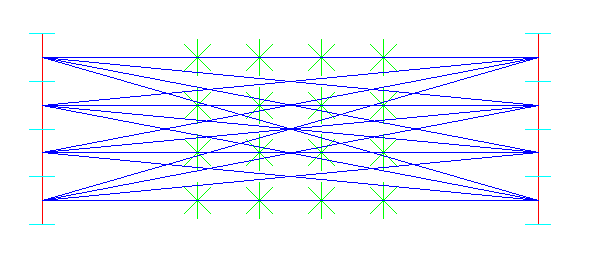
\includegraphics{images/geometry.png}
\caption{Data acquisition geometry showing: 1) voxel centers (green stars), 2) detectors (red lines) and LORs main axis (dark blue lines) \label{fig:geometry}}
\end{figure}

At this point abort the execution of the matlab script.

\subsubsection{Conventions}

In order to refer to the different voxels and detectors we will index them as follows:

Voxels (4x4 matrix):

\begin{tabular}{ c c c c }
 13 & 14 & 15 & 16\\
 9 & 10 & 11 & 12\\
 5 & 6 & 7 & 8 \\
 1 & 2 & 3 & 4 \\
\end{tabular}\\

Detectors

\begin{tabular}{ l  c  c  c  c  r}
 L4 &  &  &  &  & R4\\
 L3 &  &  &  &  & R3\\
 L2 &  &  &  &  & R2\\
 L1 &  &  &  &  & R1\\
\end{tabular}\\
where L refers to the left detector array and R to the right detector array.

Finally, LOR(1) is the LOR defined by detectors L1 and R1, LOR(2) is the one defined by detectors L1 and R2, LOR(5) is the one defined by detectors L2 and R1, ... and LOR(16) is the one defined by detectors L4 and R4

\subsection{Monte Carlo Approach}
\label{sec:monteCarlo}
The Monte Carlo method was invented by scientists working on the atomic bomb in the 1940s, who named it for the city in Monaco famed for its casinos and games of chance.  Its core idea is to use random samples of parameters or inputs to explore the behavior of a complex system or process. 

In our case we will simulate a PET scanner by creating  positrons that will produce pairs of gamma photons traveling in random directions.

Now, edit the \emph{pet\_student.m} file and:

\begin{itemize}
    \item comment all the \emph{pause()} statements. 
    \item comment the code that plot the LORs. That is,
    \begin{lstlisting} [language=matlab,lineskip={-1.0pt},breaklines=true] 
    for i = 1:numberOfLors
        plot([lors(i,1),lors(i,5)],[lors(i,2)+0.5,lors(i,6)+.5],'b');
    end
    pause()
    \end{lstlisting}
    \item Finally set the variable \emph{numEmissions} equal to 10. That is, we are going to create
    10 positrons
\end{itemize}

Now, you should see ten yellow lines that show the path followed by the ten gamma-rays pairs. Some of them will intersect one detector in both, the left and right detector arrays (3 rays in image \ref{fig:montecarlo}) and will be detected and the rest intersect only one detector (1 ray in image \ref{fig:montecarlo}) array or none (6 rays in image \ref{fig:montecarlo}) and will not be detected.

\begin{figure}[H]
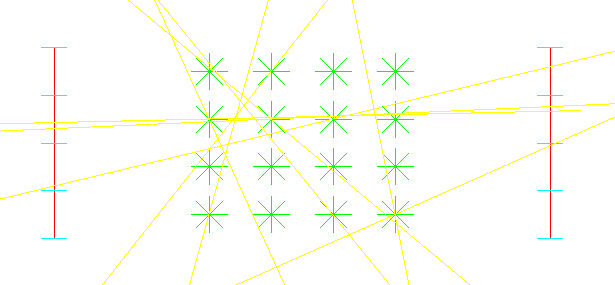
\includegraphics{images/montecarlo.png}
\caption{PET scanner showing gamma rays (in yellow) \label{fig:montecarlo}}
\end{figure}


Figure \ref{fig:0_0vs0_3} shows the result of executing the program with \emph{numEmissions} set to 1000. The blue lines represent all the gamma-ray pairs emitted by voxel(1) and that have been detected. The red lines represent all the gamma-ray pairs emitted by voxel (13)  and that have been detected.\\

\begin{minipage}{\linewidth}
\begin{framed}
\addtocounter{ejercicioNo}{1} 
Questions \arabic{ejercicioNo}: 
\begin{itemize}
   \item Using figure \ref{fig:0_0vs0_3} compute  $p(1,1)$ and $p(13,16)$. (First index represents the voxel and second the detector pair) 
   \item Are this numbers different? comment this result
   \item Repeat figure \ref{fig:0_0vs0_3} comparing voxels p(1,1) and p(6,5) (set \emph{numEmissions}  to 1000)
   \item Modify the script so the system matrix is printed and present it in your report as a 2D
   table. With these values compute $p(b,.)$. (call this script pet\_montecarlo.m)
   \item Execute the code with different values of \emph{numEmissions}. Using symmetry considerations
   (that is, taken into account which voxels  should have similar detection probabilities) select a reasonable value for \emph{numEmissions}. Report the selected \emph{numEmissions} and justify the value. 
\end{itemize}
\end{framed}
\end{minipage}

\begin{figure}[h]
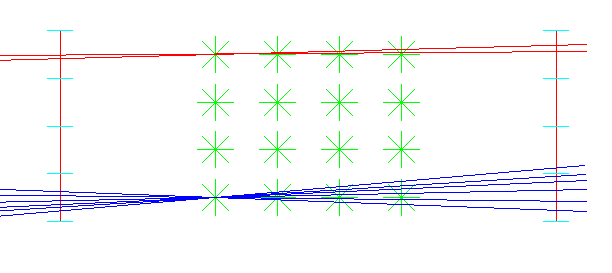
\includegraphics{images/0_0vs0_3.png}
\caption{PET scanner showing the gamma rays detected by the system and
emitted either by voxel(0) (blue) or voxel(13) (red)  \label{fig:0_0vs0_3}}
\end{figure}

\section{3D Reconstruction}

It is time to perform the 3D reconstruction. In the previous section in order to compute the system matrix and the normalization factor we have produce positrons equally distributed in space. Let us modify the matlab script so that all gamma rays are emitted from voxel(5), that is, only voxel(5) contains radiactive material. Run the program until at least one emission have been detected and them, by hand, apply equation \ref{eq:2.9}. Use as initial $\lambda$ a constant volume, that is, $\lambda(b)=1$

\begin{minipage}{\linewidth}
\begin{framed}
\addtocounter{ejercicioNo}{1} 
Questions \arabic{ejercicioNo}: 
\begin{itemize}
   \item Include in your report the value of the: system matrix and normalization factor, $\sum_{b=1}^{B}\lambda^{old}\left(b\right)p(b,d)$ and $\lambda^{new}$
   \item name the script produced for this step pet\_3dreconstruction.m.
\end{itemize}
\end{framed}
\end{minipage}


\subsection{Improving the model}
\label{sec:ImprovingTheModel}
\subsubsection{Positron free travel}
\label{sec:PositronFreeTravel}

Our model of the PET scanner is very crude 
(see \url{http://www.opengatecollaboration.org/} for a full featured PET simulator). Let us make it 
more accurate. As the radioisotope undergoes positron emission decay, it emits a positron. The emitted positron travels in tissue for a short distance (typically less than 1 mm, but dependent on the isotope), during which time it loses kinetic energy, until it decelerates to a point where it can interact with an electron. Let us model this behavior. Modify the matlab script so that photons are created not in the voxel center but in a neighborhood. This effect can be achieved by adding a small random value to the variables xp1, yp2, xp2 and yp2 that define the lines along each pair of gamma-rays travel. Modify the matlab script as described in this paragraph, use a gaussian random number generator with standard deviation = 0.25  and answer the following questions (CAUTION: do not add the same random number to all gamma rays):

\begin{minipage}{\linewidth}
\begin{framed}
\addtocounter{ejercicioNo}{1} 
Questions \arabic{ejercicioNo}: 
\begin{itemize}
   \item Repeat figure \ref{fig:0_0vs0_3} comparing voxels 1 and 11
   before and after the script modification.
   \item Include a table with the system matrix before and after the modification and comment on how does it change? The number of LORs that are able to detect a given voxel is higher or smaller than 
   before? How this will affect the reconstruction? Why? 
   \item Modify the script so the system matrix is printed and present it in your report as a 2D
   table both after and before the script modification. With these values compute $p(b,.)$ both after and before the script modification. (call this script pet\_freetravel.m)
   %\item include a copy of the modified matlab script used in this section. Named it pet2.m 
\end{itemize}
\end{framed}
\end{minipage}


\subsubsection{False Positives: random coincidences}
\label{sec:FalsePositives}

PET relays on simultaneous or coincident detection of pairs of photons moving in approximately opposite directions. Photons that do not arrive in temporal "pairs" (i.e. within a timing-window of a few nanoseconds) are ignored.
Two major sources of noise in PET are scatter (in a detected pair of photons, at least one of them was deflected from its original path by interaction with matter in the field of view, leading to the pair being assigned to an incorrect LOR) and random events (photons originating from two different annihilation events but incorrectly recorded as a coincidence pair because their arrival at their respective detectors occurred within a coincidence timing window). We will explore the effects of the latter source of noise.

So far we have assumed that our detector is so fast and the radioisotope dose so low that random coincidences can be ignored. Let us suppose that this is not the case and that in average two positrons are created in such a way that the detector cannot separate them (this assumption will produce  an unrealistic high number of random coincidences). Therefore, we need to modify the program so two gamma rays are generated at the same time. That is,  instead of having one pair of gamma rays defined by (x1p,y1p,x2p,y2p), we will have two pairs of gamma rays defined by (ax1p,ay1p,ax2p,ay2p) and (bx1p,by1p,bx2p,by2p). In order to make the programming easier, we define a ``random coincidence'' as the case in which the first gamma ray pair intersects one but not both detectors and the second pair intersects one but not both detectors. An extra constrain is that the detector array (either left or right) intersected by the first gamma ray pair should be different from the detector array intersected by the second array   

\begin{minipage}{\linewidth}
\begin{framed}
\addtocounter{ejercicioNo}{1} 
Questions \arabic{ejercicioNo}: 
\begin{itemize}
   \item Modify the original matlab script to incorporate the generation of randoms (call this script pet\_question3.m).
   \item Report on the total number of positrons generated, the number of randoms and the number of true detections. (call this script pet\_random.m)
\end{itemize}
\end{framed}
\end{minipage}


%\section{For Extra credit: PET data as Projections}
%It is possible to convert the PET list-mode data into a set of projections
%that may be used to reconstruct the specimen using a traditional method
%as FBP instead of equation \ref{eq:2.9}.\\

%\begin{minipage}{\linewidth}
%\begin{framed}
%\addtocounter{ejercicioNo}{1} 
%Questions \arabic{ejercicioNo}: 
%\begin{itemize}
%   \item Modify the original matlab script to compute projections from list-mode data (call this script pet\_question4.m).
%   \item Describe the algorithm used to convert list-mode data to a set of projections.
%\end{itemize}
%\end{framed}
%\end{minipage}



\subsection{Material to be handed no later than 1 week after the end of this assignment}

Using moodle upload a single zip file with\\
\begin{minipage}{\linewidth}
\begin{framed}

\begin{itemize}
          \item A single pdf file containing the answer to all the questions asked in this assignment as well as all the figures, tables and plots requested.
          \item All matlab scripts mentioned in the  question boxes. The scripts should be written in independent text files that can be executed from matlab directly.
      \end{itemize}
\end{framed}
\end{minipage}

NOTE: remember that the system matrix gives probabilities and therefore the sum of all its element 
cannot be greater than 1.

\bibliographystyle{ieeetr}
\bibliography{iriarte2007}


\end{document}
